 
\section{Barcelona Sensors Platform}
\label{sec:implementation_bsp}

\subsubsection*{Barcelona}

Barcelona is one of the cities that are available in the iCity platform. The
city a Barcelona has invested heavily in the Smart Cities trend. Barcelona has
opened a lot of static data in the OpenDataBCN initiative. Apart from that,
Barcelona has three platforms integrated with the iCity platform:

\begin{enumerate}
  \itemsep0em
  \item The {\bf Barcelona Sensor Platform}. This platform allows any developer
to access the data sent by sensors that are distributed around the city. This
platform includes these kind of sensors:
    \mylist
      \item Environmental sensors (temperature, $NO_2$, $CO_2$, noise, etc.).
      \item Sustainability (level of capacity of the container waste).
      \item Traffic management (parking sensors).
      \item Walkers flows (number of pedestrian).
      \item Irrigation control (ground humidity, wind rain, temperature).
    \mylistend
  \item {\bf Smartcitizen Platform}. Smart Citizen is a platform to generate
participatory processes of people in the cities.
  \item {\bf IRIS} (Complaints and Suggestions System).
\end{enumerate}

From these three possibilities I have picked the Barcelona Sensor Platform (BSP
from now on). This is because the Smartcitizen platform is in an experimental
stage and the IRIS platform is too different to the London endpoint.

\subsubsection*{Storm}

The Storm application implements the support for BSP in the {\bf
com.mssola.snacker.bsp} package. This package resides inside the
``snacker-bsp'' directory.

My original design consisted of one spout and five bolts (one for each kind of
sensor). However, I later decided that this was not realistic for the following
reasons:

\begin{enumerate}
  \itemsep0em
  \item The iCity API does not make a distinction between the type of data.
Therefore, since there is not a real distinction, the data has to be treated
equally, regardless of the type.
  \item Conceptually, multiple bolts means that we are doing completely
different things with the same raw data. For example, with the same data one
bolt could store something on the database, and another bolt could compute
something else. This is not the case.
\end{enumerate}

Thus, the final design is fairly similar to the design of the London AQS
service:

\begin{center}
  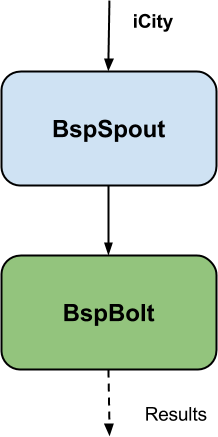
\includegraphics[scale=0.6]{implementation/images/bsp.png}
\end{center}

\begin{enumerate}
  \itemsep0em
  \item The {\bf BspSpout} fetches the raw data from the iCity platform. After
this, it cleans up the data and sends it to the BspBolt.
  \item The {\bf BspBolt} receives the data from the BspSpout and performs a
set of computations. After this, it sends the results to the given socket.
\end{enumerate}

\subsubsection*{Streaming API}

The update rate of the sensors from the BSP is not very high, but at least it
is better than London. This is why I have decided that BSP will have a
streaming API. A streaming API means that a request has the following lifecycle:

\begin{enumerate}
  \itemsep0em
  \item The API layer receives an HTTP request that points to the BSP service.
  \item The API layer subscribes to the BSP service for this request.
  \item The BSP will continously fetch and process data. The processed data
will be sent through the socket.
  \item The API layer receives data from the BSP service but does not
unsubscribe the socket. That is, it will keep on receiving data indefinitely.
  \item The API layer creates a response with ``Transfer-Encoding: chunked''.
This means that the TCP socket established between the client and the API layer
will not fade away until one of both sides decides to close the connection.
This will not happen from our end, so it is up to the client to close the
connection.
\end{enumerate}

From the client's perspective, this means that he can ``subscribe'' to an
endpoint and he will be getting updates in realtime without doing anything
special. Let us remember that this was one of the major goals of this project:
to be able to get updates of processed data on realtime.

One endpoint has been implemented for this purpose:

\begin{center}
  /bsp/s/\{id\}
\end{center}

The {\bf id} parameter has two possible values: ``all'' or a device id.
Therefore, a client has the possibility to subscribe to all the devices from
Barcelona and he will be gettings updates in realtime.
